\section{Evaluation results}
\label{sec:eva}
The performance evaluation for the different test sets can be seen in figure \ref{fig:performance}. The CoNLL performance is an average of both the ned.testa -and ned.testb set. The parliamentary item set is of the same size as ned.testa. The last column in the figure shows performance after reclassification of entity types in the parliamentary items set. Accuracy is obtained by binarily evaluating all tokens: if a token is predicted as an entity (regardless of type), but it turns out not to be, this token prediction is marked as incorrect. Tokens not seen as an entity while they are, idem. Low accuracy would be the results of Frog incorrectly identifying non-entities as entities, since the other way around would not hit accuracy hard due to the sparcity of entities in the test sets. Recall is measured as the proportion of entities retrieved that were annotated in the test set, again not looking at entity type. IOB-precision is the precision of the first part of the IOB+type tag. This will measure how well a beginning of an entity consisting of multiple tokens is found, or how different entities following each other are seperated. Type precision also looks at the IOB+type tag, but with exclusion of the IOB part. Regular precision is the combination of type-precision en IOB-precision. F-measure is the harmonic mean of the regular precision and the recall.

\begin{figure}
\begin{tabular}{c||c|c|c|}
     & \textbf{CoNLL} & \textbf{Parliamentary items} & \textbf{Parliamentary items + reclassification} \\\hline \hline
Accuracy & 0.950 & 0.973 & 0.974 \\\hline
Recall & 0.845 & 0.906 & 0.908\\\hline 
IOB-precision & 0.915 & 0.890 & 0.890 \\\hline 
Type-precision & 0.672 & 0.616 & 0.662\\\hline 
Precision & 0.629 & 0.563 & 0.603\\\hline
F-measure & 0.720 & 0.694 & 0.725\\\hline
 \end{tabular}
\caption{Performance overview of both sets}
\label{fig:performance}
\end{figure}

Since type-precision has appeared to be relatively low, it would be interesting to analyze errors made per type. Figure \ref{fig:confusion} shows a prediction distribution for each type.
It can be seen that location as a type is predicted very accurately, while prediction of the type person seems to be significantly more difficult.

\begin{figure}
    \centering
    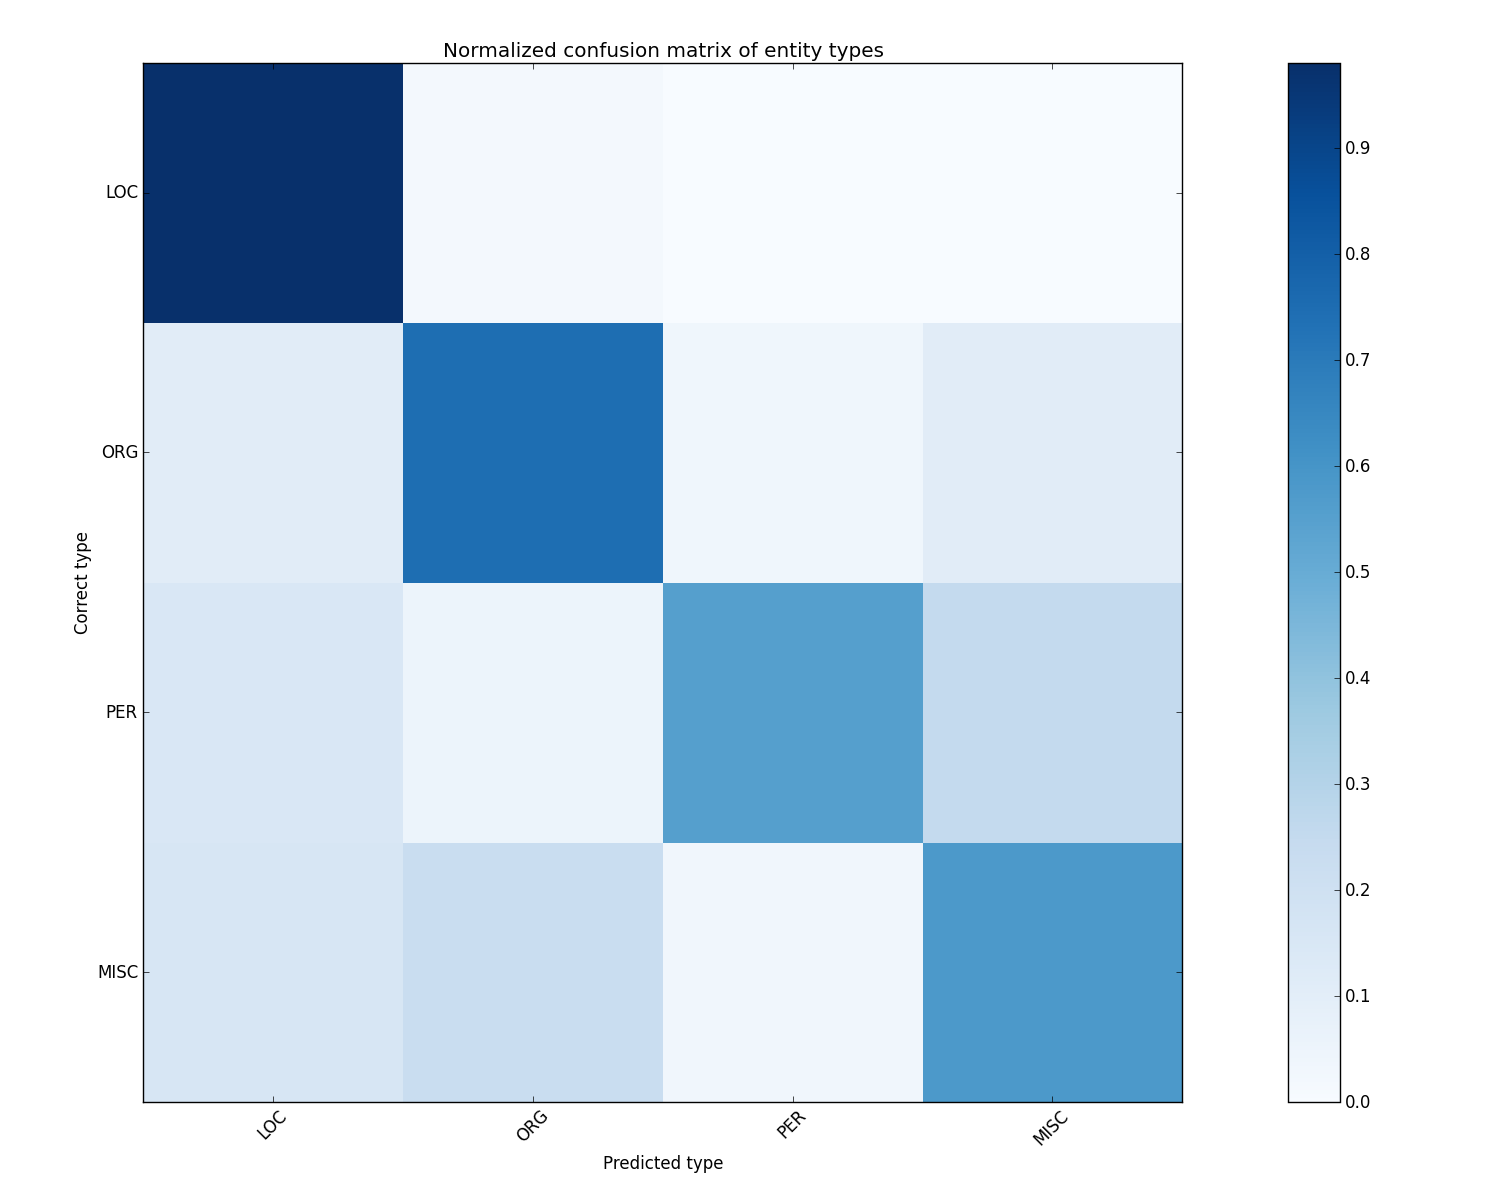
\includegraphics[scale=0.4]{fig/confusion_matrix_reclassified}
    \caption{Prediction distribution per type}
    \label{fig:confusion}
\end{figure}
